\documentclass[french]{article}
\usepackage[T1]{fontenc}
\usepackage{fullpage}
\usepackage{babel}
\usepackage{hyperref}
\usepackage{graphicx}
\usepackage[justification=centering]{caption}
\usepackage{amsmath}
\usepackage{amssymb}

\hypersetup{
  colorlinks=true,
  linkcolor=black,
  urlcolor=blue
}

\graphicspath{ {./img/} }
\title{%
    \huge Prédire les changements climatiques  \\
    \bigskip
    \large E2 - Cas pratique \\ 
    Développeur en Intelligence Artificielle,
    titre professionnel enregistré au RNCP - École IA Microsoft by Simplon}
\date{12 février 2024}
\author{par Vincent Papelard}

\begin{document}
    \renewcommand{\contentsname}{Table des Matières}
    \maketitle
    \pagenumbering{arabic}
    \pagenumbering{gobble}
    \newpage
    \tableofcontents
    \newpage
    \pagenumbering{arabic}

    \section*{Introduction}
    Un grand organisme de prédiction météorologique nous contacte. Afin de prédire au mieux l'évolution du climat à échelle mondiale dans le but de sensibiliser la population au réchaffement climatique, ses dirigeants souhaitent remplacer leurs modèles de prédiction vieillissant par un modèle d'IA moderne, en cherchant la meilleure précision possible. Ils nous demandent par ailleurs de leur fournir les instructions nécessaires à la mise en place et l'utlisation de ce modèle.
    Le code associé à ce dossier est disponible \href{https://github.com/vinpap/predict_climate_change}{sur GitHub}.

    \addcontentsline{toc}{section}{Introduction}
    \section{Jeu de données de test}
    Afin de faire la démonstration du modèle retenu, on utilisera \href{https://www.kaggle.com/datasets/berkeleyearth/climate-change-earth-surface-temperature-data}{ce dataset}, qui rencense les températures mensuelles moyennes sur Terre depuis le XVIIIè siècle, à échelle mondiale et en des points du globe spécifiques. Ce jeu de données est issu de l'aggrégation d'une grande quantité de données historiques réalisée par l'ONG \href{http://berkeleyearth.org/about/}{Berkeley Earth}, une ONG affiliée au Lawrence Berkeley National Laboratory, un laboratoire universitaire de Californie.
    On s'intéressera plus spécifiquement à la température mensuelle moyenne sur Terre de 1860 à nos jours. Cette information est stockée dans la table GlobalTemperatures.csv, qui se présente comme ceci :
    
    \begin{figure}[h]
        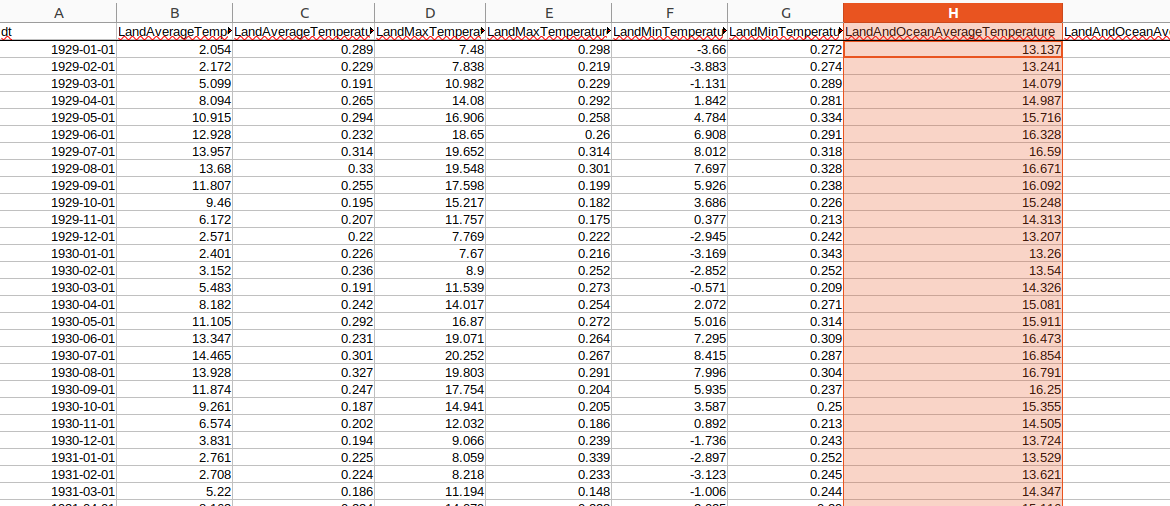
\includegraphics[width=12cm]{dataset}
        \centering
        \caption{Table GlobalTemperatures.csv}
        \centering
    \end{figure}

    Les prédictions seront réalisées avec les données de la colonne "LandAndOceanAverageTemperature" (en surbrillance sur la figure), qui recense la température moyenne en degrés Celsius sur Terre chaque mois, au-dessus des continents comme des océans. Nous disposons ainsi d'environ 2000 valeurs, dont les premières remontent à 1850.
    \section{Modèles de prédiction envisagés}

    Il existe de nombreux modèles d'IA qui permettent de réaliser des prédictions à partir de séries temporelles. Dans la mesure où il est impossible de tous les traiter, il a fallu faire des choix. Après recherches, les trois modèles qui seront comparés dans ce dossier sont :
    \begin{itemize}
        \item \textbf{ARIMA}
        \item \textbf{Facebook Prophet}
        \item \textbf{Réseaux LSTM (Long Short-Term Memory)}
    \end{itemize} 
    
    Ces modèles ont été spécifiquement choisis car ils sont largement utilisés et il existe beaucoup de littérature scientifique à leur sujet. Il nous sera ainsi possible de nous baser sur la littérature scientifique existante pour choisir, parmi ces modèles, le plus adapté à nos besoins. Le fonctionnement de chaque modèle est abordé dans la section suivante.

    \subsection{ARIMA (Autoregressive Integrated Moving Average)}

    Plus qu'un modèle, ARIMA est une combinaison de plusieurs modèles :
    \begin{itemize}
        \item \textbf{AR - Autorégression} : ce composant calcule la valeur d'une variable à partir des $p$ dernières observations, $p$ étant un paramètre de notre modèle. Si l'on note $X_t$ la valeur de notre variable à un instant $t$, on a donc :

        \begin{equation}\forall t : X_t = \sum_{i=1}^p \alpha_i X_{t-1} + \epsilon_t \end{equation}
        avec $\epsilon$ l'erreur et $\alpha_1,...\alpha_p$ des réels.
        \item \textbf{MA - Moyenne Mobile} : la moyenne mobile (Moving Average en anglais) exprime une valeur à un instant $t$ comme une combinaison linéaire de $q$ erreurs passées :

        \begin{equation}\forall t : X_t = \epsilon_t + \sum_{i=1}^q \alpha_i \epsilon_{t-i} \end{equation}

        Pour modéliser des séries temporelles de façon plus complexe, on combine le modèle AR et le modèle MA pour créer un modèle dit "ARMA" :

        \begin{equation}\forall t : X_t = AR_t + MA_t = \sum_{i=1}^p \alpha_i X_{t-1} + \epsilon_t + \sum_{i=1}^q \beta_i \epsilon_{t-i} \end{equation}
        avec $\alpha_1,...\alpha_p$ et $\beta_1,...\beta_p$ des réels.
        \item \textbf{I - Intégration} : Le modèle ARMA a une limitation : \textbf{il ne peut modéliser que des séries de donneées stationnaires, c'est-à dire sans tendance à la baisse ou à la hausse}. Pour régler ce problème, on ajoute la composante I au modèle ARMA.
        Cette composante élimine les dépendances des données au temps en différenciant la série temporelle, c'est-à-dire en travaillant avec $X_t - X_{t-1}$ au lieu de $X_t$. Cette différenciation est réalisée $d$ fois, $d$ étant un paramètre de notre modèle ARIMA. 

    \end{itemize}

    En plus des paramètres $p$, $q$ et $d$ présentés ci-dessus, le modèle ARIMA a aussi un paramètre $m$ qui définit la saisonnalité des données, s'il y en a une. Dans la mesure où nous travaillons avec des moyennes de température mensuelles, cette valeur $m$ vaut 12 dans notre cas.
    
    \subsection{Facebook Prophet}

    \href{https://facebook.github.io/prophet/}{Facebook Prophet} est un modèle de prédiction sur des séries temporelles proposé par Meta. 
    Pour réaliser des prédictions, Facebook Prophet considère les données comme la combinaison additive de quatre composants : 
    \begin{itemize}
        \item la tendance
        \item la saisonnalité annuelle
        \item la saisonnalité hebdomadaire
        \item une liste de jours feriés importants fournis par l'utilisateur.
    \end{itemize}
    Chacune de ces composantes est gérée par un modèle distinct. La saisonalité annuelle, par exemple, est modélisée à l'aide de séries de Fourier.
    Facebook Prophet se veut simple à mettre en place et permet de réaliser des prédictions très rapidement. Ce modèle était à l'origine développé pour être utilisé avec les données commerciales auquelles sont confrontés les data scientists de Meta, ce qui le rend plus adapté à certains types de données spécifiques (données financières ou commerciales par exemple). 
    
    \subsection{Réseaux LSTM (Long Short-Term Memory)}

    Le terme "LSTM" désigne un type de réseau neuronal récurrent (RNN). Les LSTM ont été créés pour pallier aux problèmes de disparition (ou d'explosion, selon les cas) du gradient souvent rencontrés lorsque l'on utilise un réseau récurrent pour traiter de longues séquences de données.
    Par rapport aux RNN classiques, les LSTM ajoutent au réseau un composant supplémentaire qui garde une mémoire de long terme, par opposition à la propagation d'informations naturellement présente dans les RNN via la réutilisation des sorties précédentes en tant que valeurs d'entrée. Les LSTM comportent des composants logiques appelés "gates" qui déterminent quels éléments doivent être stockés dans cette mémoire de long terme.

    
    \begin{figure}[h]
        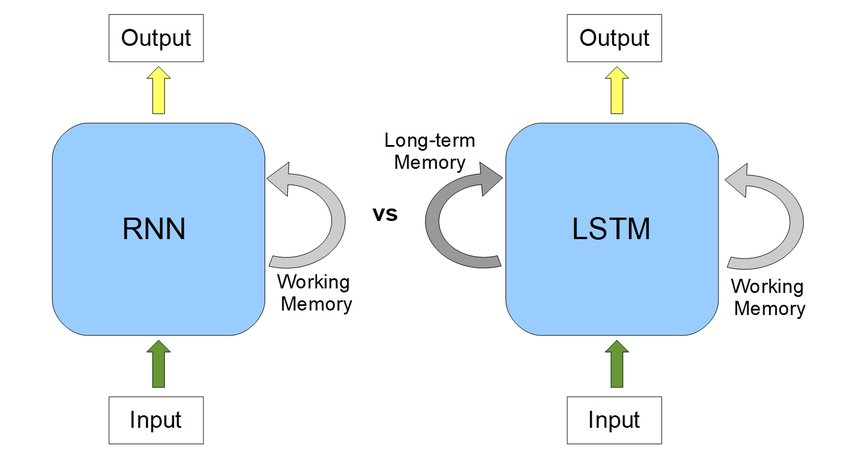
\includegraphics[width=12cm]{RNNvsLSTM}
        \centering
        \caption{Représentation d'un LSTM}
        \centering
    \end{figure}

    Loin d'être propres aux séries temporelles, les LSTM sont utilisés pour répondre à de nombreux problèmes tels que la traduction automatique ou la génération de langage naturel.

    \section{Comparaison des modèles}

    \subsection{Présentation des sources}

    Les comparaisons ci-dessous s'appuient sur les travaux publiés dans des publications scientifiques et des sites web spécialisés dont la liste complète est disponible dans la bibliographie. Parmi ceux-là, on pourra notamment citer :
    \begin{itemize}
        \item \href{https://repository.tudelft.nl/islandora/object/uuid:29fcfb96-3e96-4b11-93ec-217ba69ea412/datastream/OBJ/download}{Cette étude} de la Delft University of Technology qui compare les trois modèles pour la prévision de traffic 
        \item \href{https://arxiv.org/pdf/2107.12770.pdf}{Cette comparaison} d'ARIMA, de Facebook Prophet et de modèles combinant le LSTM à des CNN, par l'Université de Perugia. Ces modèles sont appliqués à la prédiction de prix de vente de produits alimentaires
        \item \href{https://neptune.ai/blog/arima-vs-prophet-vs-lstm}{Cet article} du fournisseur de soutions de MLOps Neptune.ai qui compare les performances de ces modèles sur des données boursières.
    \end{itemize}

    \subsection{Conclusions des sources choisies}
    Bien que toutes les sources n'arrivent pas à un consensus évident, on peut tout de même en dégager plusieurs conclusions.
    Dans leur étude réalisée à l'Univesité de Perugia sur les prix de vente de produits alimentaires, Lorenzo Menculini et al. arrivent aux conclusions suivantes en comparant les performances des trois modèles :
    \begin{itemize}
        \item  Facebook Prophet produit des prédictions moins précises que les LSTM et ARIMA. Cependant, le modèle s'avère très simple et rapide d'utilisation, sans avoir besoin de beaucoup de nettoyage préalable sur les données.
        \item Les LSTM ont les meilleurs performances des trois modèles testés, mais aussi un temps d'entraînement largement plus long.
        \item ARIMA a une précision supérieure à Facebook Prophet et inférieure au LSTM, mais un temps d'entraînement très court comparé à ces derniers.
    \end{itemize}
    Voici les performances calculées pour chaque modèle dans le cadre de cette étude. On remarquera que les modèles ont été testés sur trois produits différents :
    RMSE obtenue pour chaque modèle :
    \begin{center}
        \begin{tabular}{ |c| c| c| c| }
            Produit & 1 & 2 & 3 \\
            ARIMA & cell1 & cell2 & cell3 \\ 
            LSTM & cell4 & cell5 & cell6 \\  
            Facebook Prophet & cell7 & cell8 & cell9    
        \end{tabular}
    \end{center}

    \end{document}